% !TEX root = catron-dissertation.tex
\epstopdfsetup{outdir=./images/07_multiple_sensor_filtering/}

\chapter{Combination of Filters}
\label{chap:07_multiple_filter}
% \textcolor{red}{
%   \begin{itemize}
%     \item Figure 7.2 - ylabel OPDRMS(t)
%     \item Figure 7.3,7.4 - Backward Moving Filter
%     \item Add figure showing the combined Velocity_LSE_MSPOD multidimensional spectrum
%   \end{itemize}
% }

The previous chapter investigated a series of filters that were applied in a singular fashion to a set of optical wavefronts.
This chapter will discuss combining several of these filters together in series.


\section{Velocity and LSE-SPOD Filter}
In addition to the LSE-SPOD filter using all 16 additional sensors that was shown in Chapter \ref{chap:06_single_filter}, a velocity filter was applied to the wavefront first.
Table \ref{tab:07_lse_mspod_table_vel} shows the summary of these filters when used separately or together.
The LSE-SPOD was shown previously to remove vibration noise from wavefront measurements with an approximately 85\% reduction in $\opdrms$ at Mach of 0.3 \cite{DeLucca-2014-RAJvGdv7}.
Similar results were observed using the combination of optical tip/tilt removal and LSE-SPOD on both single dimension (temporal) and multidimensional spectra.
Optical tip/tilt removal alone accounted for a 78.6\% reduction in $\opdrms$, with a combination of 16 microphones and accelerometers and the LSE-SPOD bringing the reduction in $\opdrms$ to 83.9\% at Mach of 0.3.
The combination of tip/tilt removal and the velocity filter showed a greater reduction of 82.3\%.
At a Mach number of 0.5, the use of optical tip/tilt removal, the velocity filter, and 16 sensors in LSE-SPOD, the $\opdrms$ was brought down to 0.0181 $\mu m$ and stilled showed a significant amount of narrow-band signals (see Figure \ref{fig:07_lse_spod} and \ref{fig:07_lse_mspod}).
This is about a 30\% reduction when compared with the other filters used in Table \ref{tab:08_filter_summary}, and represents almost entirely an additional reduction in contamination to the aero-optical signal by removing the broadband disturbances.
This was also significantly above the estimated $\opdrms$ of 0.0142 $\mu m$ for the $M=0.6$ case (See Section \ref{sect:02_BL_OPD} and \cite{Gordeyev-2014-jcJndkHM}).
\begin{table}
  \centering
  \caption{$\opdrms$ ($\mu m$) comparison of using LSE-MSPOD filtering process when combined with a velocity filter.}
  \input{../matlab/07_multiple_sensor_filtering/lse_mspod_table_vel.txt}
  \label{tab:07_lse_mspod_table_vel}
\end{table}

With the LSE-SPOD method the more sensors that were used in the filtering process the greater the reduction in the $\opdrms$, as can be seen in Figure \ref{fig:08_lse_summary}.
\begin{figure}
  \centering
  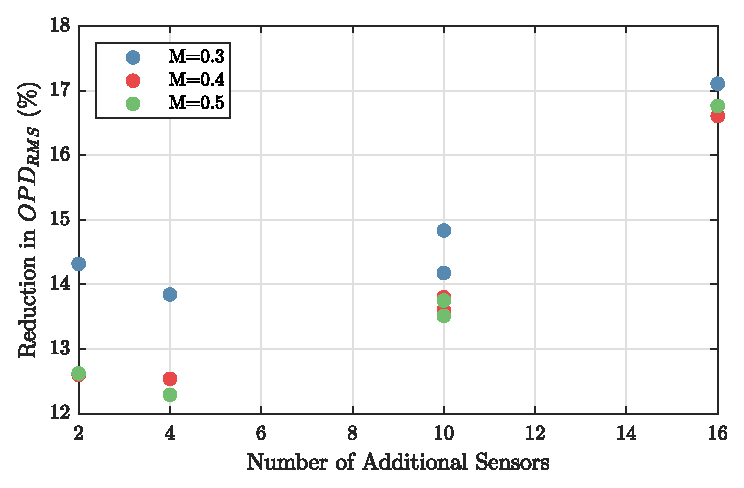
\includegraphics{../matlab/08_conclusion/lse_summary.eps}
  \caption{Percent reduction in $\opdrms$ from the tip/tilt removed case using LSE-SPOD filtering.}
  \label{fig:08_lse_summary}
\end{figure}
The combination of the DAQ and preamplifier used for the duct-mounted microphones had a significantly lower dynamic range when compared to the other sensors, possibly leading to a diminished reduction in the performance of the four-sensor filtering.
The signal reduction using all 16 sensors was fairly uniform with frequency, as shown in Figure \ref{fig:08_lse_mspod_freq}.
\begin{figure}
  \centering
  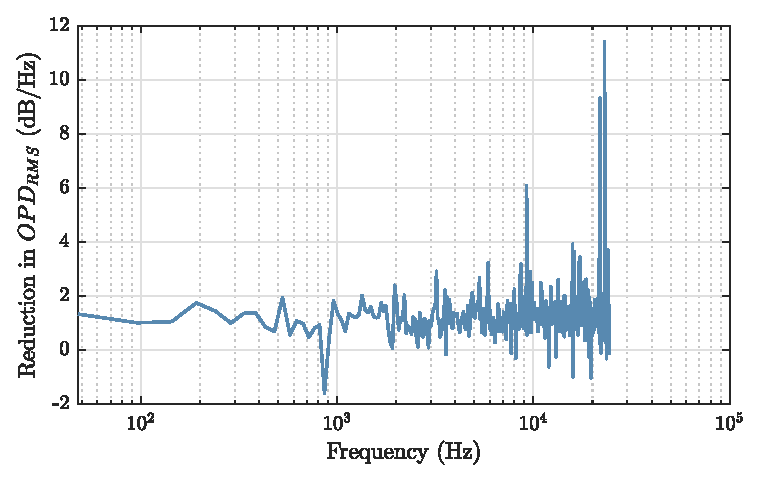
\includegraphics{../matlab/07_multiple_sensor_filtering/lse_mspod_freq.eps}
  \caption{Reduction in $\opdrms(t)$ as a function of temporal frequency using 16 sensors with LSE-SPOD in the M=0.5 case when compared to tip/tilt removal.}
  \label{fig:08_lse_mspod_freq}
\end{figure}
On average there was a 1.3dB/Hz reduction in the $\opdrms$ with slight peaks at some of the significant narrow-band signals.
At the blade-passing frequency (517 Hz) there was a 2dB/Hz reduction and for the narrow-band signals around 3 and 6 kHz there was a 3dB/Hz reduction.
The first, second, and third harmonics of the blade-passing frequency, at 1034 Hz, 2068 Hz, and 4136 Hz, had a below average reduction in the signal.

While the use of additional sensor measurements to aid in filtering of optical wavefront measurements using LSE-SPOD showed little benefit in this study (at least compared to the single sensor filtering techniques), it could show significant benefit in future measurements.
Specifically, for measurements with models that are likely to create narrow-band signal noise, additional sensor information could be used in conjunction with a baseline filter for determining which narrow-band signals that need to be retained in the spectrum.


\section{Backward, Velocity, and Baseline Filter}
Among the filters discussed, three are useful for isolating aero-optical signals from a wavefront.
The first of these is a filter for separating the portion of the optical disturbances that are moving either upstream or downstream to the flow (Section  \ref{chap:06_up_down_filter}).
An undesirable effect of this filter is that it may remove some of the aero-optical signal, which can happen to the boundary-layer signal\footnote{These low frequency aero-optical disturbances may be a combination of the outer boundary layer and free-stream turbulence.} at low temporal frequencies.
The second useful filter is the low-pass velocity filter which preserves the signal that is moving within a narrow velocity range (Section \ref{chap:06_velocity_filter}).
The third is the baseline estimator (Section \ref{chap:06_baseline}), which removes the narrow-band signals associated with the blade-passing frequency and its harmonics, the mean-lensing component, and other temporally narrow-band signals.
However, some of these removed narrow-band signals could include part of the aero-optical signal of the wind-tunnel model.

Figure \ref{fig:08_dispersion_filters} shows the multidimensional spectra of the output of these three filters individually plus the spectra of these three filters combined.
\begin{figure}
  \centering
  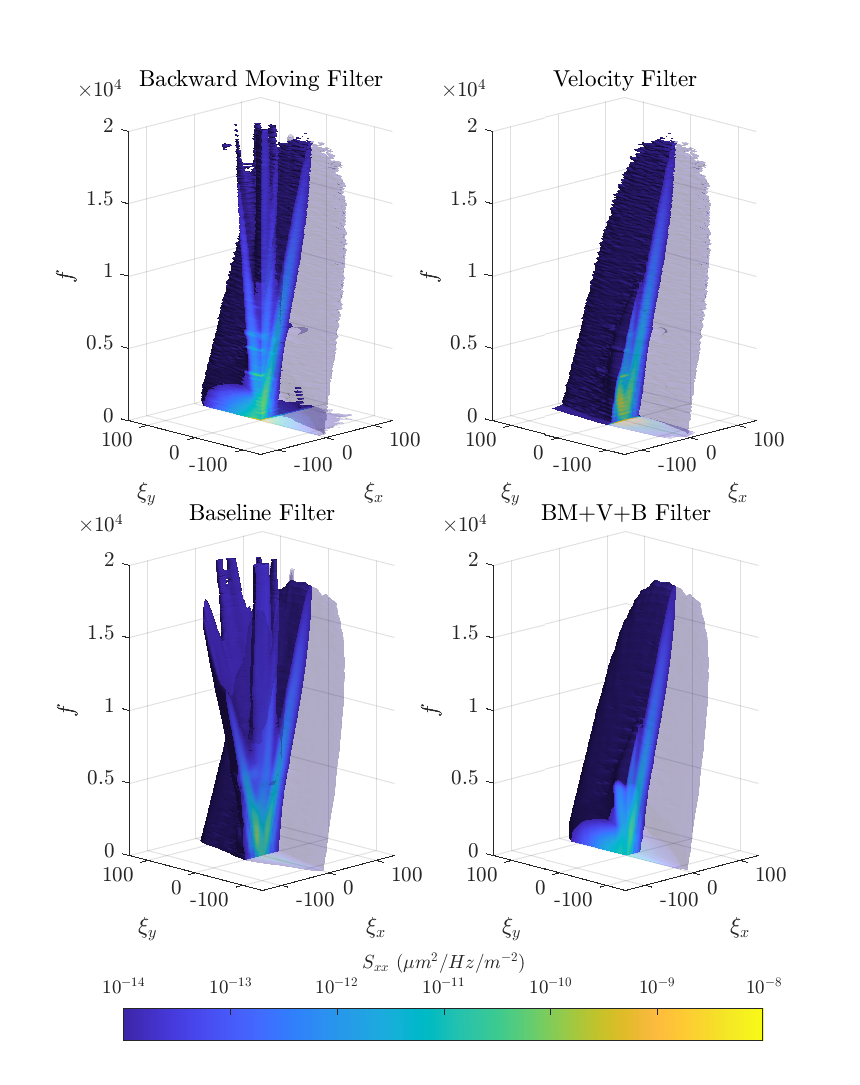
\includegraphics{../matlab/08_conclusion/dispersion_filters.eps}
  \caption{Multidimensional spectra of three single sensor filtering techniques and a combination filter.}
  \label{fig:08_dispersion_filters}
\end{figure}
The backward moving filter, that removes all upstream-moving disturbances (Figure \ref{fig:08_dispersion_filters} top left), does remove some of the boundary-layer signal at low temporal frequencies.
The portion of the acoustic cone and stationary modes that are on the downstream-moving portion of the spectrum are retained.
The velocity filter (Figure \ref{fig:08_dispersion_filters} top right) removes most of the broadband signal from the various noise sources.
There is a portion of the acoustic cone and stationary modes that intersect or lay near the boundary-layer signal that is slightly attenuated, producing a slight hump on the upstream-moving side of the boundary-layer that extends up to about 10 kHz and along the $\xi_y$ axis over the range of about $\pm25\ m^{-1}$.

The baseline filter (Figure \ref{fig:08_dispersion_filters} bottom left) removes all of the temporal narrow-band signals including the mean-lensing portion of the spectra.
The noisy surface of the spectra is removed which also eliminates some the boundary-layer aero-optical signal.
The combination filter (Figure \ref{fig:08_dispersion_filters} bottom right) applies the velocity and backward moving filter to the baseline filter.
This filter loses some of the boundary-layer signal due to the noisy surface being smoothed out and the portion that crosses into the upstream-traveling portion of the spectrum.
The portion of the acoustic cone and stationary modes that is the most contaminating in the velocity filter is removed due to the backward moving and baseline filter.

A zoomed in slice of the multidimensional spectra is shown in Figure \ref{fig:08_dispersion_filters_slices} for the horizontal moving plane waves.
\begin{figure}
  \centering
  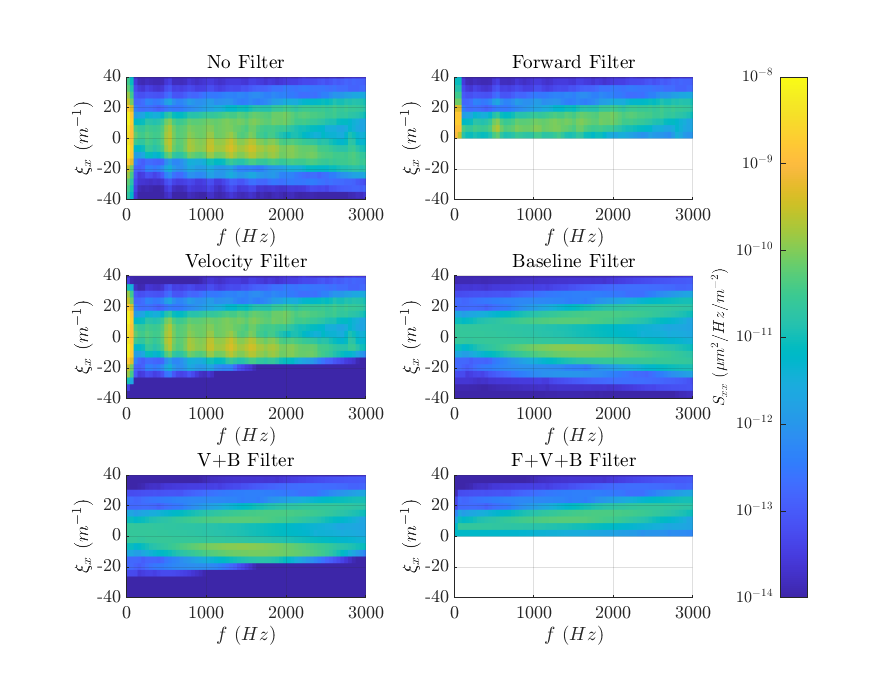
\includegraphics{../matlab/08_conclusion/dispersion_filters_slices.eps}
  \caption{Multidimensional spectral slices for the various single sensor filtering techniques showing the horizontal moving plane waves.}
  \label{fig:08_dispersion_filters_slices}
\end{figure}
A large portion of the signal contamination happens at the blade-passing frequency and its harmonics as well as in the mean-lensing region.
This contamination is present in all of the multidimensional spectra that do not utilize the baseline filter.
Even with the velocity filter there is significant contamination on the upstream-moving portion of the spectra due to these narrow-band signals as well as due to the presence of the acoustic cone and stationary modes.
While the backward moving filter removes some of the boundary-layer signal it removes significantly more of the noise signals that would otherwise be present in the spectra with just the velocity and baseline filters applied.

Representative wavefronts were generated from these multidimensional spectra using the same process as generating a synthetic wavefront from the synthetic spectra in Chapter \ref{chap:05_synthetic} in order to calculate the $\opdrms$.
Table \ref{tab:08_filter_summary} shows the $\opdrms$ values for the various filters used in Figure \ref{fig:08_dispersion_filters_slices}.
\begin{table}
  \centering
  \caption{Summary of single sensor filters}
  \input{../matlab/08_conclusion/dispersion_filters.txt}
  \label{tab:08_filter_summary}
\end{table}
Both the backward moving and baseline filters reduced the $\opdrms$ of the wavefront a similar amount of 36 and 40\% respectively.
The velocity filter only reduced the $\opdrms$ a small amount of 8.5\% due to the retention of the strongest portion of the narrow-band signals.
The combination of the velocity and baseline filters reduced the $\opdrms$ of the wavefront by 46\% but those still retain a significant portion of the acoustic cone and stationary mode signal.
By combining these three single sensors filters, the $\opdrms$ was reduced 58\% but this is likely under the true value due to some loss of the boundary-layer signal from the backward moving filter at low temporal frequencies and the removal of the fluctuations from the baseline filter.
There could be some narrow-band signals that would be generated by a model that would be removed with this filtering scheme.
The estimated $\opdrms$ from Gordeyev \cite{Gordeyev-2014-jcJndkHM} (Equations \ref{eqn:02_opdrms_gor} and \ref{eqn:02_opdrms_gor_fit}) is $0.0142\ \mu m$ for a double boundary layer, which puts the velocity and baseline filter combination in good agreement.
